% TODO
% Add footnotes
% Print this pdf

\documentclass [12pt, letterpaper, twoside] {article}
\usepackage[utf8]{inputenc}
\usepackage [left=1.0in, right=1.0in, top=1.0in, bottom=1.0in] {geometry}
% For keeping time
\usepackage {datetime}
% For pictures/graphs
\usepackage {tikz}
% The essential math library
\usepackage {amsmath}
% To make tables
\usepackage {tabu}
% To add multiple rows or columns per table column/row
\usepackage {multirow}
% To add horizontal lines spanning only some columns in tables
\usepackage {array}
\usepackage {verbatim}
% To add captions to tables
\usepackage {caption}
\usepackage {float}
% For the degree symbol
\usepackage {gensymb}
% To make graphs
\usepackage {pgfplots}
% To insert images
\usepackage {graphicx}

\raggedbottom
\begin {document}
\begin {titlepage}
\begin {center}
Department of Biological, Chemical, and Physical Science\\
\vspace {0.1cm}
Illinois Institute of Technology\\
\vspace {0.1cm}
General Physics I: Mechanics (PHYS 123-02)\\
\vspace* {\fill}
\begingroup
\Large
\textbf {Angular Momentum}
\vspace {0.35cm}

\normalsize
Lab 12
\vspace {1.5cm}
\endgroup
\vspace* {\fill}
\end {center}

\vspace*{\fill}
\begin {flushright}
\footnotesize
Emily Pang, Coby Schencker (lab partner)\\
Date of experiment: 14 Nov 2019\\
Due date: 21 Nov 2019\\
Lab section L04\\
TA: Mithila Mangedarage\\
Updated \usdate\today~(\currenttime)
\end {flushright}
\end {titlepage}

\begin {table}[h!]
  \centering
  \begin {tabular} {| l | r | r | r | r |}
    \hline\hline
    & Mass (kg) & Inner Radius (m) & Outer Radius (m) & I (kg\(\cdot\text{m}^2\))\\
    \hline
    \multirow{3}{*}{Disk} & 1.3918 & & 0.1140 & 0.009044 \\ %916 (LDR)
    & 1.3918 & n/a & 0.11375 & 0.009004 \\ %294
    & 1.3917 & & 0.1139 & 0.009027 \\ %408
    \hline
    Average & 1.3918 & & 0.1139 & 0.009025 \\ %66667 (LDR) %83333 (LDR) %199
    \hline
    \multirow{3}{*}{Hoop} & 1.4233 & 0.05355 & 0.06375 & 0.004933 \\ %919 (LDR)
    & 1.4233 & 0.05350 & 0.06345 & 0.004902 \\ %954 (LDR)
    & 1.4233 & 0.05355 & 0.0635 & 0.004910 \\ %28
    \hline
    Average & 1.4233 & 0.05353 & 0.06357 & 0.004915 \\ %3333 %6667 (LDR) %038
    \hline
    Average \(I_{total}\) (kg\(\cdot{\text{m}}^2\)) & & & & 0.01394 \\ %0237
    \hline\hline
  \end {tabular}
  \caption {General Mass and Dimension Measurements}
\end {table}

\begin {table}[h!]
  \centering
  \begin {tabular}{| l | r | r | r |}
    \hline\hline
    & \(m_{1}\) & \(m_{2}\) & \(m_{3}\) \\
    \hline
    \multirow{3}{*}{Mass (kg)} & 0.0499 & 0.0900 & 0.1499 \\
    & 0.0500 & 0.0899 & 0.1499 \\
    & 0.0500 & 0.0899 & 0.1499 \\
    \hline
    Average & 0.0500 & 0.0899 & 0.1499 \\ %66667 (LDR) %33333
    \hline
    \multirow{3}{*}{Angular acceleration (\(\tfrac{\text{rad}}{\text{s}^2}\))} & 0.497 & 1.02 & 1.82 \\
    & 0.514 & 1.02 & 1.82 \\
    & 0.508 & 1.02 & 1.82 \\
    \hline
    Average & 0.506 & 1.02 & 1.82 \\ %333333
    \hline
    \multirow{3}{*}{Moment of inertia (kg\(\cdot\text{m}^2\))} & 0.0178 & 0.0157 & 0.0146 \\ %33979 %72784 (LDR) %29663
    & 0.0173 & 0.0157 & 0.0146 \\ %78696 (LDR) %5538 (LDR) %29663
    & 0.0175 & 0.0157 & 0.0146 \\ %82776 (LDR) %5538 (LDR) %29663
    \hline
    Average & 0.0175 & 0.0157 & 0.0146 \\ %31817 %61181 (LDR) %29663
    \hline\hline
  \end {tabular}
  \caption {Experiment 1 Hanging Masses and Angular Accelerations}
\end {table}

\begin {table}[h!]
  \centering
  \begin {tabular} {| l | r | r | r |}
    \hline\hline
    Trial & 1 & 2 & 3 \\
    \hline
    \(w_{\text{i}}\) (\(\tfrac{\text{rad}}{\text{s}}\)) & 7.549 & 8.683 & 17.119 \\
    \hline
    \(I_{\text{total,i}}\) (kg\(\cdot{\text{m}^2}\)) & 0.009025 & 0.009025 & 0.009025 \\ %199 %199 %199
    \hline
    \(w_{\text{f}}\) (\(\tfrac{\text{rad}}{\text{s}}\)) & 4.291 & 4.218 & 10.239 \\
    \hline
    \(I_{\text{total,i}}\) (kg\(\cdot{\text{m}^2}\)) & 0.01394 & 0.01394 & 0.01394 \\ %0237 %0237 %0237
    \hline
    \(\Delta{L}\) (kg\(\tfrac{\text{m}^2}{s}\)) & -0.008314 & -0.01957 & -0.06209 \\ %67 (LDR) %5883 %3369
    \hline
    \(\Delta{KE}_{\text{rot}}\) (J) & -0.1288 & -0.2162 & -0.5917 \\ %22749 %16103 %35979
    \hline\hline
  \end {tabular}
  \caption{Experiment 2 Conservation of Angular Momentum}
\end {table}

\noindent
Our lab consisted of a rotation platform with a disk and hoop, three metal balls, various weights, a string, a rotating ramp, and a rotation sensor. For the first experiment, the moment of inertia was observed using the disk and hoop. The second experimented examined the conservation of angular momentum with three metal balls and the rotating ramp.

\subsection* {Question 1}

PART A \\\\
The equation for a disk and cylindrical tube (hoop) using the parallel axis theorem is as follows:
\begin {equation*}
  \begin {split}
    I_{total} = \dfrac{1}{2}M_{\text{disk}}R_{\text{disk}}^2 + \dfrac{1}{2}M_{hoop}(R_{\text{inner}}^2 + R_{\text{outer}}^2) \\
  \end {split}
\end {equation*}
The calculated moments of inertia for the disk and hoop are shown in Table 1. \\

\noindent
PART B \\\\
We use the following equation to compare the experimental and calculated moments of inertia:
\begin {equation*}
  \begin {split}
    \tau &= I\alpha \\
    I &= \dfrac{\tau}{\alpha} \\
    I &= \frac{mgr}{\alpha} \\
  \end {split}
\end {equation*}

\noindent
The radius at which the gravity force of the hanging mass was applied at was 0.018125 m. This data is not recorded in any of the tables as it is a value from the previous lab (we forgot to obtain this value). Our experimental values in Table 1 are close to the expected values in Table 2, showing that the moments of inertia equations hold for the torque equation. \\


\noindent
PART C \\\\
The conservation of angular momentum states the following when there are no external torques:
\begin {equation*}
  \begin {split}
    \vec{L}_{i} &= \vec{L}_{f} \\
    I_{i}w_{i} &= I_{f}w_{f} \\ 
  \end {split}
\end {equation*}
Table 3 shows the change in angular momentum between the disk and the hoop. We calculated the moment of inertia of the disk as 0.009 kg\(\cdot\text{m}^2\) as shown in Table 1, which was used for the initial moment of inertia. Table 3 also shows the change in kinetic energy. By definition, in elastic collisions, the kinetic energy is conserved, which we do not see in our results. Thus, the collision between the disk and hoop is inelastic.

\subsection* {Question 2}
In the single ball experiment, we saw that after the rail slowed down enough for the metal ball to roll down, the angular velocity increased and then slowed down again as it did before. 

\begin {figure}[h!]
  \centering
  \includegraphics[width=100mm,scale=0.5]{first.jpg} %width=\linewidth
  \caption {Single ball rolling down}
\end {figure}

\noindent
For the experiment involving three metal balls, we saw that as the rail slowed down enough, one metal ball rolled down and the rail's angular velocity increased as it rolled down. This occurred for each metal ball until all of the balls had rolled down. We see this in Figure 2 where the velocity slowly decreased and jumped suddenly at around \(t = 22\) seconds. 

\begin {figure}[h!]
  \centering
  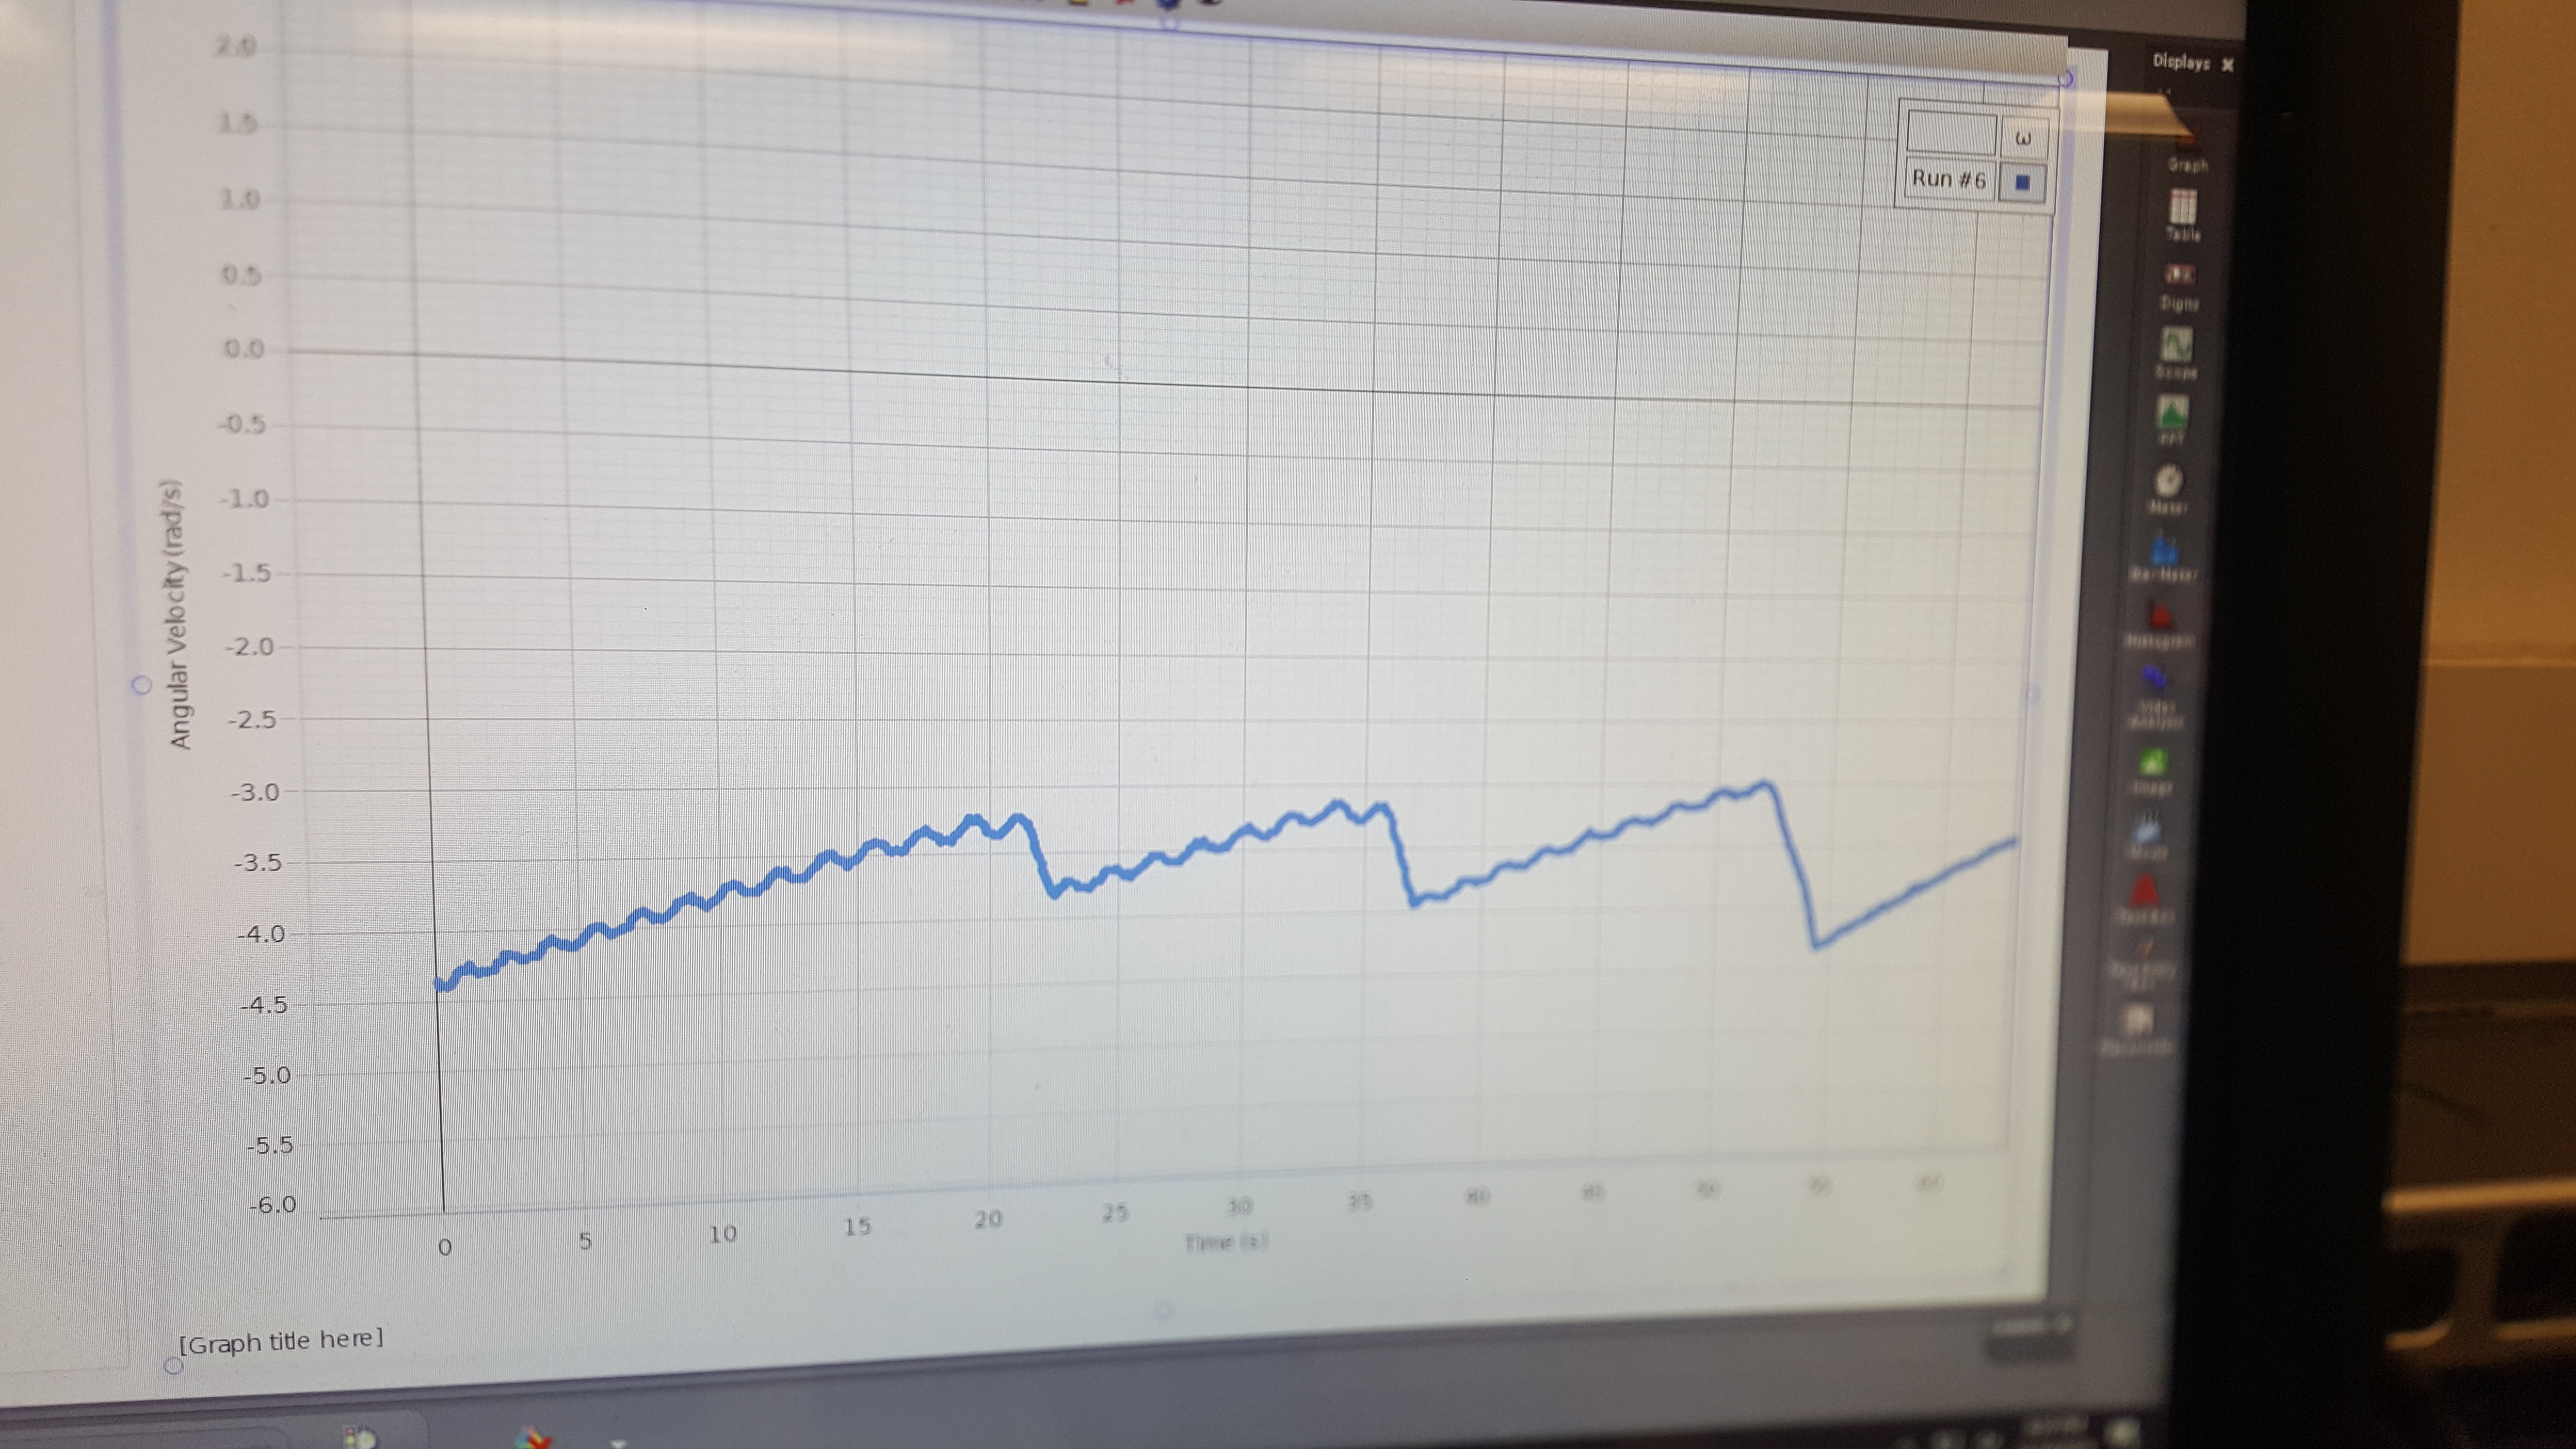
\includegraphics[width=100mm,scale=0.5]{second.jpg}
  \caption {Three balls rolling down}
\end {figure}

\noindent
Angular momentum is conserved when there are no external torques. Since the act of the balls rolling down did not exert a torque, the angular momentum stayed the same. As each ball rolled down, it decreased the moment of inertia, increasing the angular acceleration (from a negative slope to a positive slope).
\begin {equation*}
  \begin {split}
    \alpha = \dfrac{mg}{I} \\
  \end {split}
\end {equation*}

\noindent
Note: The angular velocity was recorded as negative during these experiments.
\end {document}
